\documentclass[aspectratio=169]{beamer}
\usepackage{standalone}

\usepackage{stmaryrd}
\usepackage{listings}
\usepackage{fontawesome}
\usepackage{bm}

\def\examplecite#1{{\textit{\color{black!60!blue}\small Example from \cite{#1}}}}


\usepackage[hyperref=auto,style=alphabetic,backend=bibtex]{biblatex}
\addbibresource{kwarcpubs.bib}
\addbibresource{extpubs.bib}
\addbibresource{extcrossrefs.bib}
\addbibresource{bib.bib}
\usepackage{appendixnumberbeamer}
\usepackage{tikz}
\usepackage{tikz-qtree}
\usetikzlibrary{arrows.meta}
\usetikzlibrary{shapes}
\usetikzlibrary{mmt}
\usetikzlibrary{docicon}

\usetheme{Pittsburgh}
% \setbeamertemplate{footline}[frame number]
\setbeamertemplate{footline}{\hfill\insertframenumber\,/\,\inserttotalframenumber\quad\strut}
\setbeamertemplate{navigation symbols}{}
\usecolortheme{beaver}
\setbeamertemplate{frametitle}[default][left]
% \setbeamersize{text margin left=3em}

\usepackage{utils/colors}
\usepackage[forbeamer]{utils/basic}
\usepackage{utils/operators}
\usepackage{utils/mylstmisc}
\usepackage{utils/lstmmt}

\lstset{basicstyle=\ttfamily}
\lstset{commentstyle=\itshape\color{commentfont}}

\title{AnnoTize: A Flexible Annotation Tool for Documents with Mathematical Formulae}


% rdf nodes
\tikzset{urinode/.style={draw, ellipse, minimum width=1.3cm, minimum height=0.6cm}}
\tikzset{typenode/.style={draw}}
\tikzset{bnode/.style={draw, ellipse, minimum width=1.0cm, minimum height=0.6cm}}
\tikzset{literal/.style={draw, rounded corners=0.1cm}}

% rdf edges
\tikzset{normaledge/.style={-Latex}}
\tikzset{typeedge/.style={arrows={-Latex[open]}}}

% custom nodes
\tikzset{body/.style={fill=green!50}}
\tikzset{target/.style={fill=blue!30}}
\tikzset{annotation/.style={fill=red!50}}


\author{Lukas Panzer \and \textbf{Jan Frederik Schaefer}}
\institute{FAU Erlangen-N\"urnberg/KWARC}
\date{\textbf{MathUI Workshop}\\Cambridge, UK\\September 7, 2023}

\begin{document}
\frame\titlepage


\begin{frame}
    \frametitle{Natural Language Processing and Mathematical Language}
    \begin{itemize}
        \item Natural language processing has benefitted from a long tradition of annotation tasks and benchmarks
        \item STEM documents pose problems:
            formulae, tables, \textellipsis
            \com{not really unicode strings}
        \item Why care?\\
            $\leadsto$ Semantic services
    \end{itemize}
\end{frame}


\begin{frame}
    \frametitle{Motivation: semantic services}
    \faSearch\;\; $\bm{1.5\,\text{\bf eV}}$
    \\[1em]
        \quad\quad\faExternalLink\;\; $1.43 \pm 0.9\,\text{eV}$\\[1em]
        \quad\quad\faExternalLink\;\; $2.4 \cdot 10^{-19}\,J$

    \vspace{3em}
    \faSearch\;\; $\bm{\sum_{k=-\infty}^\infty \text{\bf exp}(-\pi k^2)}$
    \\[1em]
        \quad\quad\faExternalLink\;\; $\sum_{n=-\infty}^\infty e^{-\pi n^2} = \ldots$
\end{frame}


\begin{frame}
    \frametitle{Motivation: semantic services}
    \hfill \examplecite{krisciunas2022including}\par
    \centering
    \begin{tikzpicture}
    \node at (0, 0) {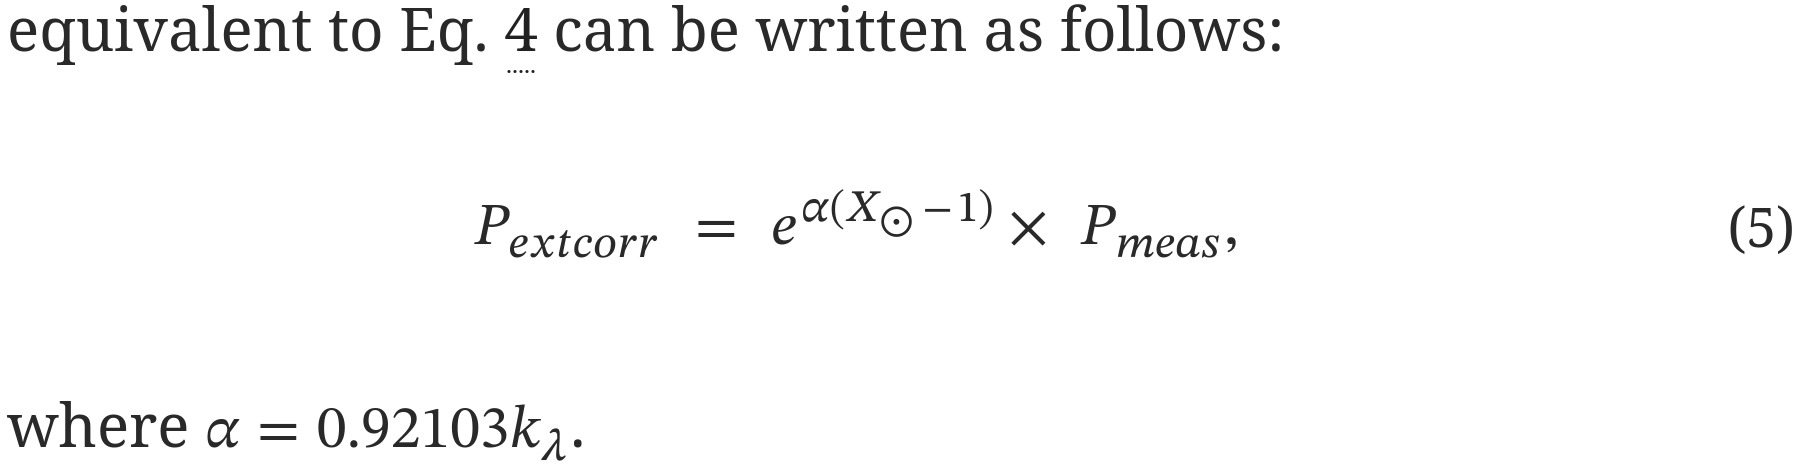
\includegraphics[width=0.8\textwidth]{extcorr_2107.02876.png}};
    \onslide<2>{\node at (1.6, -1.6) {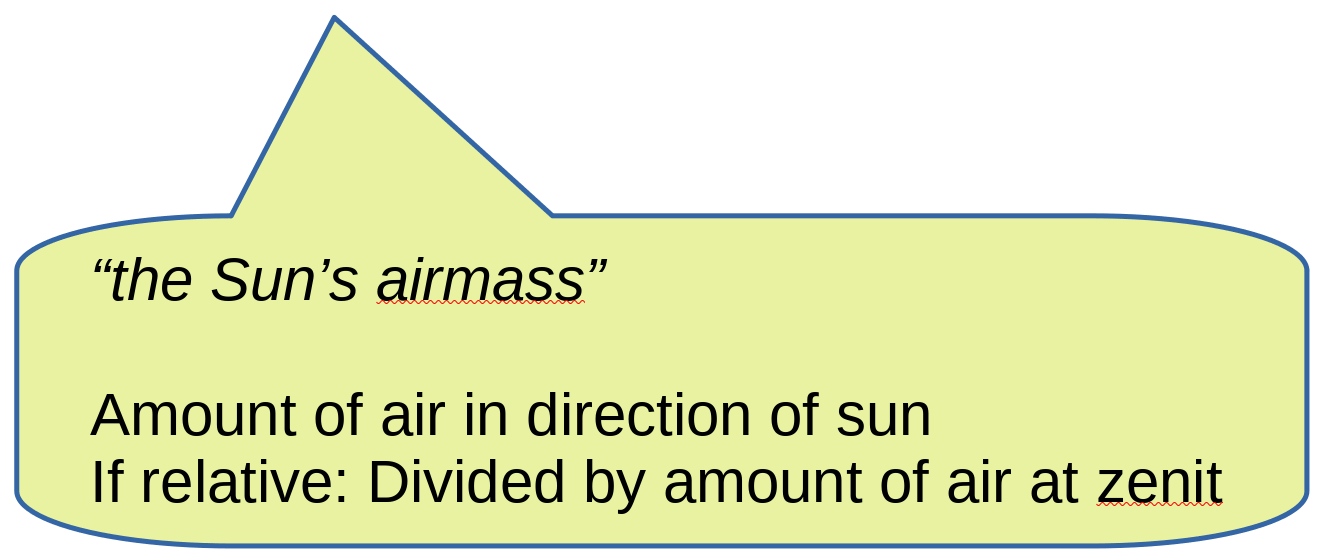
\includegraphics[width=0.5\textwidth]{bubble.png}};}
    \onslide<3>{\node at (1.5, -2.1) {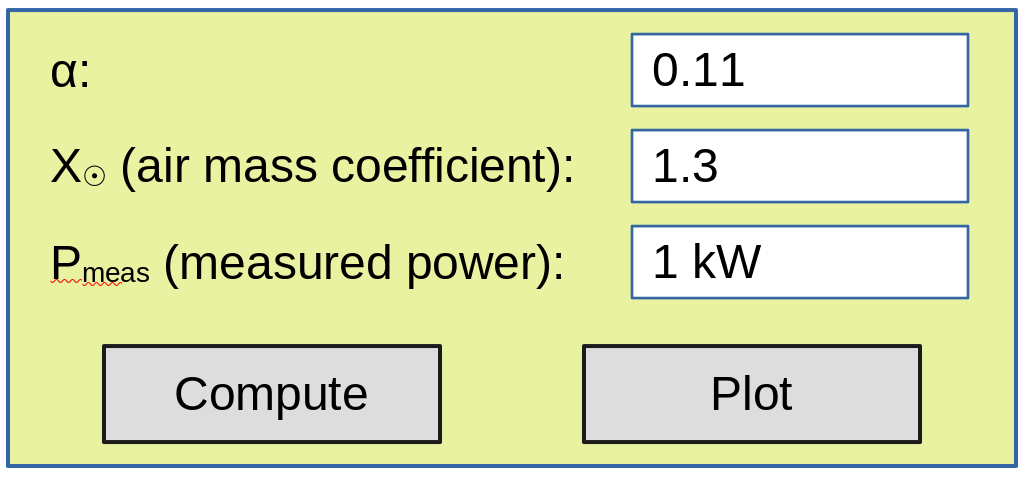
\includegraphics[width=0.5\textwidth]{compute.png}};}
    \end{tikzpicture}
%     \begin{itemize}
%         \item Computable formulae
%         \item Screen readers
%         \item Active documents
%         \item Formula search
%     \end{itemize}
\end{frame}


\begin{frame}
    \frametitle{Motivation: semantic services}
    \centering
    \Large
    For all those services\\
    {\bfseries we need semantic annotations!}\\\com{(full formalization not necessary)}
    \vspace{2em}\par
    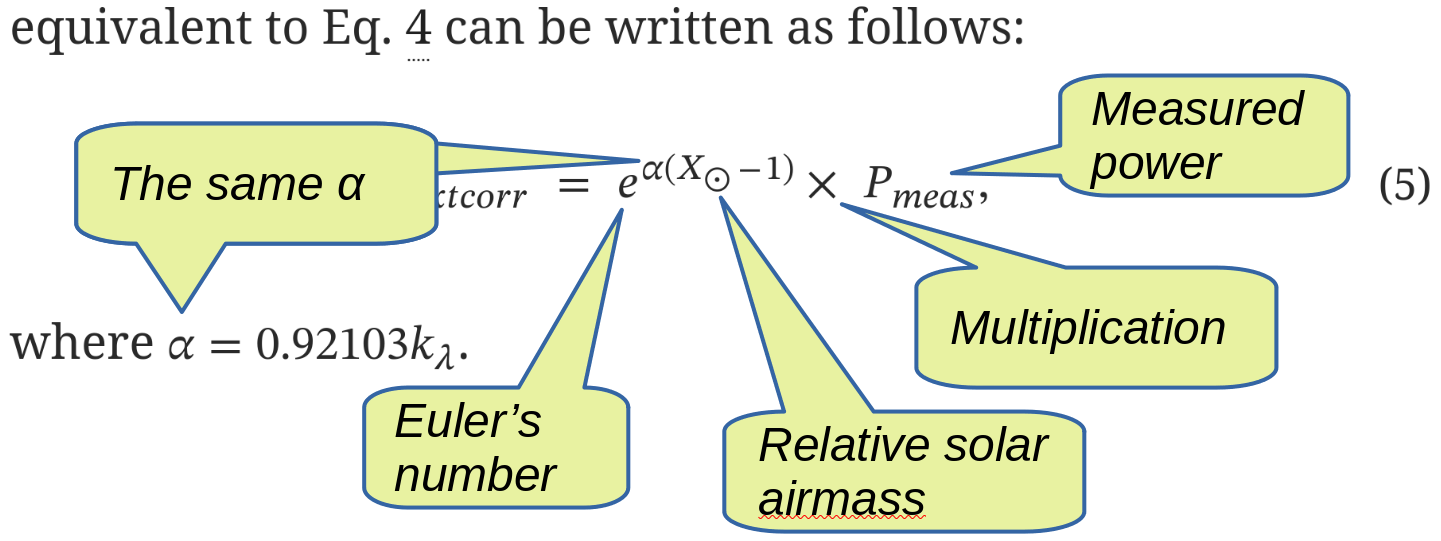
\includegraphics[width=0.5\textwidth]{annos.png}
    \vspace{2em}\par
    \pause
    Authors don't provide them $\leadsto$ We have to infer them
\end{frame}





\begin{frame}
    \frametitle{AnnoTize}
    {
        \centering
        \textbf{We will need manual annotations}
        \\\com{for evaluation and possibly training}
        \vspace{2em}\par
        Formulae prevent us from using the standard tools
        \\\com{no reasonable plaintext representation}
        \vspace{2em}\par
        $\leadsto$ We present \textbf{AnnoTize}, a flexible annotation tool for math documents\\\com{\url{https://github.com/rezakul/AnnoTize}}
    }
\end{frame}


\begin{frame}
    \frametitle{Challenge: Formulae}
\end{frame}


\begin{frame}
    \frametitle{}
\end{frame}


\begin{frame}[allowframebreaks,t]
    \frametitle{References}
    \printbibliography
\end{frame}

\end{document}
